Criptography overlaps constantly with cybesecurity: they share a lot of
common fields of study and the same keen objective of making secrets.
\begin{key}{Cryptography}
    Cryptography is, from greece kryptos + graphein, the \textbf{art of secret
    writing}: it has been used mostly for commercial and military interests.
\end{key}
Examples of criptated messages exist from the moment writing was invented
(writing itself was a form of secrecy): there existed several physical
ciphers in past times that had lots of vulnerabilites. They could be
\textbf{stolen}, the secret was \textbf{shared} (so if i stole this secret
his friend would not know that i am \textbf{faking} to be his friend) and
once an enemy figured out said secret he can \textbf{read past messages}.
The best solution would be to \textbf{change the secret}, but from now on
the enemy knows how the secret is formed and will try to \textbf{brute 
force it}. 
In the real world we must assume that all threat agents know the algorithm used
to encrypt the messages: the only thing that is left unknown is the key.
Kerckhoffs, a matematitian, stated the principles for a good cipher, some
of them are:
\begin{itemize}
    \item It must be practically (if not mathematically) unbreakable
    \item The key must be communicable without written notes and changeable
    whenever the correspondant want
    \item \textbf{It should be possible to make it public, even to the enemy}
\end{itemize}

The latter is justified by how in modern times information travels way faster 
than we can imagine and by the fact that major algorithms are known: ultimately
we can arrive at the same conclusion.
\begin{key}{Kerckhoffs' Principle}
    The security of a cryptosystem relies only on the secrecy of the key and
    \textbf{never} on the secrecy of the algorithm
\end{key}
We will see how, even by knowing what's going on under the hood of a system,
sometimes we will never be able to decrypt a message.

\begin{key}{Data}
    Data is defined in cryptography as the union of:
    \begin{itemize}
        \item \textbf{Plaintext space} - the set of possible messages, usually
        $\{ 0,1\}^l$ where $l$ is the length of the message
        \item \textbf{Ciphertext space} - the set of possible ciphertext, 
        usually $\{ 0,1\} ^{l'}$ where usually $l' \ge l$
        \item \textbf{Key space} - the set of possible keys, usually 
        $\{ 0,1\}^\lambda$ where $\lambda$ is the length of the key
    \end{itemize}
\end{key}

\begin{key}{Functions}
    The functions used in cryptography are:
    \begin{itemize}
        \item \textbf{Encryption Function} - P x K $\rightarrow$ C
        \item \textbf{Decryption Function} - C x K $\rightarrow$ P
    \end{itemize}
\end{key}

There are several types of attacks made to break a cryptosystem:
\begin{itemize}
    \item \textbf{Ciphertext only attacks} - when the analyst has only 
    ciphertext
    \item \textbf{Known plaintext attack} - when the analyst has a set of
    pairs plaintext-ciphertext
    \item \textbf{Chosen plaintext attack} - analyst can choose plaintexts 
    and obtain their respective ciphertexts
\end{itemize}
\begin{warning}{}
    Remember: those attacks are used by criptographers to check whether a 
    cipher is secure or not, not by cybersecurity analysts. 
\end{warning}

\subsection{Perfect Ciphers and Shannon's Theorem}
Another mathematitian that contributed to the world of cryptography is 
\textbf{Shannon}, that demonstrates how unbreakable ciphers exist: 
they are called \textbf{perfect ciphers} and rely on the uniqueness of the
key for each transaction. 
\begin{key}{Perfect Cipher}
    If we define $P(M=m)$ as the probability of observing a message $m$ by an
    attacker and $P(M=m|C=c)$ as the probability that once observed a 
    ciphertext $c$ the message was actually $m$, we can define a 
    \textbf{perfect cypher} as one that has:
    \begin{equation}
        P(M=m|C=c) = P(M=m)
    \end{equation}
\end{key}
This actually means that an external observer that watches $m$ learns 
\textbf{nothing}: the bad news is that this definition is 
\textbf{non-constructive} (we don't know what a perfect cipher looks like), 
but we can imagine that to give away zero informations about our message
we need a new key \textbf{every time a new message is sent}. Shannon theorized
how a perfect cipher looks like and put it into a theorem.
\begin{key}{Shannon's Theorem}
    Any symmetric encryption is perfectly secure if
    \begin{itemize}
        \item every key is used with probability $\frac{1}{|k|}$
        \item a unique key always maps a plaintext with a unique ciphertext
    \end{itemize}
\end{key}
An example of a perfect cipher is the \textbf{XOR} cipher: given a message
$m$ and a key $k$ where $|m| = |k|$, we can cipher the message by doing
$m$ XOR $k = c$. If the listener wants to read back the message he can use
the same $k$ by doing $m = c$ XOR $k$. This method works and by randomly using
a different $k$ every time it is a perfect cipher, however the problem now lies
in \textbf{how do we send the key}: this is a crucial problem in security and
\textbf{symmetric encryption} and makes this type of ciphers 
\textbf{hardly usable}. But we can draw some practical conclusions to this 
theorem: we need to find a way to \textbf{encript a message with a function 
using this key}, the function needs to be so hard to reverse it that it would 
take lots of effort (possibly more than $O(poly(\lambda))$). 
Finally, what we need to do as cryptographers of today is:
\begin{itemize}
    \item Define the ideal attacker behaviour
    \item Assume a hard given computational problem (discrete logs, nonlinear
    boolean equations, large integers factoring, etc)
    \item Prove that any non ideal attacker solves said hard problem
\end{itemize}

Even with a perfect cipher, the system is breakable:
a system is deemed \textbf{broken} if an attacker can guess the message without
solving the hard problem and with a probability that is better than 
\textbf{random}. 

\subsection{CSPRNG}
In reality, it is good practice to exchange a \textbf{single key} that 
is \textbf{kept} and \textbf{used like  a seed} to generate \textbf{new keys}:
the concept of generating new keys involves functions and permutations that
need \textbf{randomness}. It's difficult to generate randomness in the real 
world of determinism, so we will need a complex algorithm that ensure enough
randomeness that can be called \textbf{pseudorandom}.
\begin{key}{CSPRNG}
    A \textbf{Cryptographically Safe Pseudorandom Number Generator} is a 
    deterministic function that starts from our key $\{0,1\}^\lambda$ and 
    generates something longer $\{0,1\}^{\lambda + l}$, with $l$ being the
    \textbf{stretch}, and that cannot be used to guess the key again in at 
    least $O(poly(\lambda))$ time.
\end{key}
\begin{warning}{Testing the Efficiency of a CSPRNG}
    We cannot prove that a function is solvable over $\{0,1\}^{\lambda + l}$ time
    because else we could prove that $P \ne NP$! In order to verify the 
    security and the randomness of a CSPRNG we will need to \textbf{test it}
    with time and trials.
\end{warning}
In reality we only have \textbf{candidate CSPRNGs}, we have no proof that this
function exists since we cannot prove that the function itself is solvable 
above $\{0,1\}^{\lambda + l}$ time: we use structures and libraries that 
historically tend to create good algorithms and pesudorandom numbers, one
building block that is used are called \textbf{PRPs} 
(Pseudo Random Permutations) and themselves are generated by \textbf{PRFs}
(Pseusorandom Functions).

\subsubsection{PRF}
Considering the set of all functions that map a starting sequence 
$\{0,1\}^{in}$ to a finite-length encription $\{0,1\}^{out}$ and calling
it $F$, we can say that the actual \textbf{cardinality} of this set is 
calculated as $|F| = (2^{out})^{2^{in}}$. \newline
If we have for example $F = \{f:\{0,1\}^2\rightarrow\{0,1\}^1\}$ we will have
$(2^1)^{2^2}$ = 16 possible entry tables to map every input string to a 
possible output string: since this cardinality \textbf{explodes} for big 
enough $in$ and $out$, we can use a mechanism to generate a pseudorandom 
function to select one of those functions so that it's going to be hard to
correctly guess what is the actual function between all the possible ones. 
\begin{key}{Pseudorandom Functions}
    A Pseudorandom Function is $f:\{0,1\}^{in}\rightarrow\{0,1\}^{out}$
    that uses as input the input string and a $\lambda$ bit seed and gives
    as output a sequence of characters.
\end{key}

\subsubsection{PRP}
The idea is the same as a random function, but the length of the input is 
the same as the length of the output and the action of permutation depends
totally on the key that is given to the PRP. 
\begin{key}{Pseudorandom Permutations}
    A Pseudorandom Permutation is a $p: \{0,1\}^{len}\rightarrow \{0,1\}^{len}$
    and can be seen as a bijective function that uses as input the input 
    string and a $\lambda$ bit seed and gives as
    output a permutation of the input string.
\end{key}
Real world PRPs are made by taking small bijective functions $f$ and by 
repeating the step of inserting the input and key with its output: 
by computing $f$ several times (until we are satisfied) we can obtain an 
arbitrairly complex function. In real world since we cannot prove that it takes 
$O(poly(\lambda))$ time to break the cipher, we \textbf{test them}. Nowadays 
PRPs are called \textbf{block cyphers}, the current standard block cypher was 
made through a competition. But when a cipher is to be considered \textbf{broken}? 
When it is possible to take a shortcut that is better than bruteforcing, that
is finding a solution in less than $2^{\lambda}$ attempts: this is why $\lambda$
needs to be a large number, the key \textbf{must be big enough}. 
In the real world, the current AES (Advanced Encryption Standard) 
actually uses 128, 192 and 256bits long keys and takes inputs of 256bits: 
the problem is that we have to figure out a way to divide the message in 
parts so that the key still is longer than the actual block of input. 

\subsection{Repetitions and CTR}
Since the input message is necessarily longer than the key we need to find a 
way to divide the message into chunks of text: the most basic thing we can 
imagine is to divide the message into parts and use a CSPRNG to cipher every 
chunk individually.
\begin{figure}[H]
    \centering
    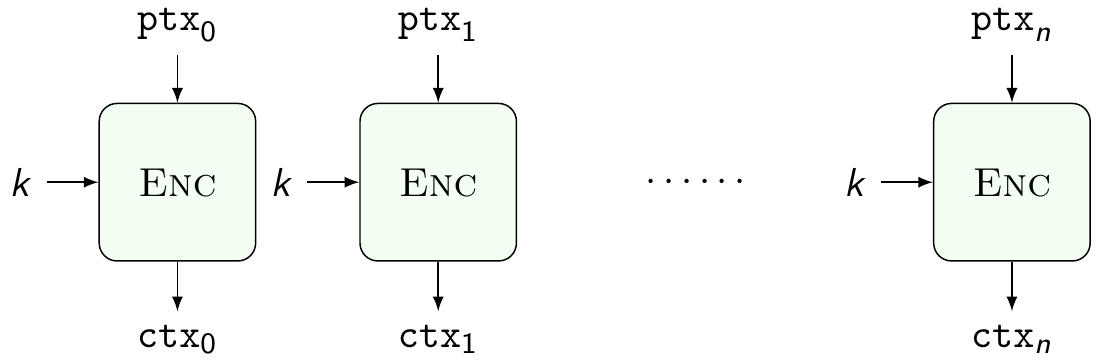
\includegraphics[width=0.8\textwidth]{Images/6Chunks.png}
\end{figure}

Actually this method is pretty \textbf{dangerous}: by coding and decoding 
single chunks everytime using the same key $k$ we could give hints to a 
possible attacker, since the ciphertext could contain repetitions and patterns.
What we can do is to implement a mechanism that uses \textbf{additional} 
variable information to encode equal chunks in the same message differently,
one solution is to develop a \textbf{counter} and a new encryption function
that takes not only the input message and the key $k$, but also said counter. 
\begin{figure}[H]
    \centering
    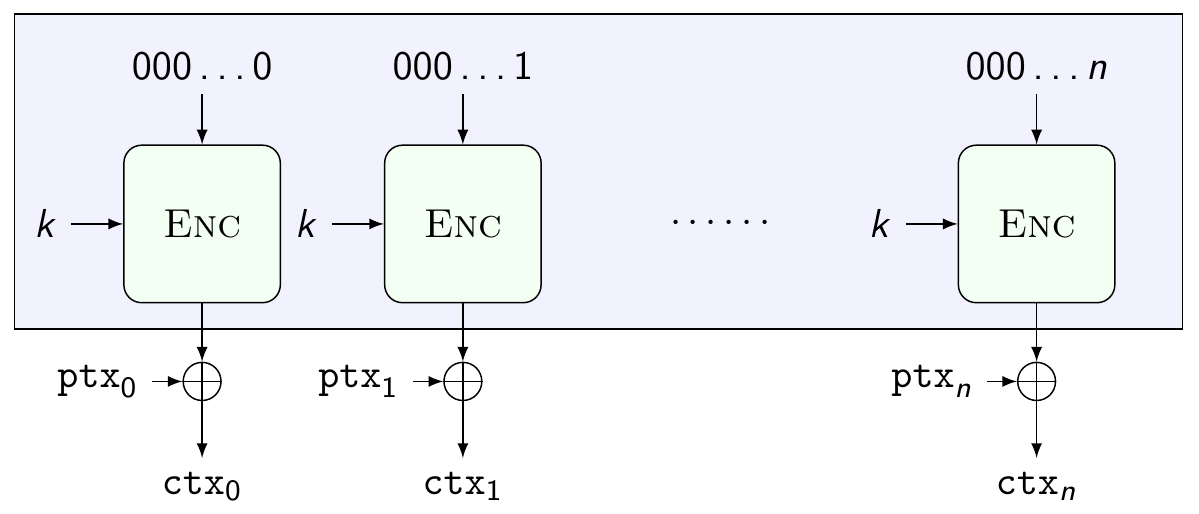
\includegraphics[width=0.9\textwidth]{Images/5CTX.png}
\end{figure}